\documentclass[11pt,a4paper]{article}
\usepackage[a4paper, margin=1.3in]{geometry}
\usepackage{mathtools}
\usepackage{fancyhdr}
\usepackage{mathrsfs}

\newcommand{\sheetNr}{12}

\pagestyle{fancy}
\fancyhf{}
\lhead{AI Planning}
\rhead{Exercise Sheet \sheetNr}
\lfoot{Axel Perschmann, Tarek Saier, \today}
\rfoot{Page \thepage\ of \pageref{lastpage}}
\renewcommand{\headrulewidth}{0.3pt}
\renewcommand{\footrulewidth}{0.3pt}
\setlength\parindent{0pt}
\newcommand{\h}[0]{\text{--}}

\begin{document}
\begin{center}
\Huge{\textbf{AI Planning}}\\
\LARGE{\textbf{Exercise Sheet \sheetNr}}
\end{center}
\vspace{2cm}
\begin{tabular}{ll}
Date: & \today\\
Students: & Axel Perschmann, Tarek Saier
\end{tabular}

\section*{Exercise 12.1}
$D^{bwd}_0:=\{\gamma\}$ \hphantom{tabtab} //per definition\\
$D^{bwd}_1:=\{\gamma,o_1\}$ \hphantom{tabtab} //$a$ is precondition, $b$ is an effect in any case\\
$D^{bwd}_2:=\{\gamma,o_1,o_2\}$ \hphantom{tabtab} // $a$ is an effect in any case\\
$D^{bwd}_3:=\{\gamma,o_1,o_2,o_3\}$ \hphantom{tabtab} //$\neg a\land b$ is an effect in any case\\
$\delta^{bwd}_G(I')=3$

\section*{Exercise 12.2}
Definitions:\\
$img_o(s)=\{s'\in S\text{ }|\text{ }s\stackrel{o}{\to}s'\}$\\
$wpreimg_o(T)=\bigcup_{s\in T}\{s\in S\text{ }|\text{ }s\stackrel{o}{\to}s'\}$\\
$spreimg_o(T)=\{s\in S\text{ }|\text{ }\exists s'\in T:s\stackrel{o}{\to}s'\land img_o(s)\subseteq T\}$\\
\\
The definition of a weak preimage can be reformulated as follows:\\
$wpreimg_o(T)=\{s\in S\text{ }|\text{ }\exists s'\in T:s\stackrel{o}{\to}s'\}$\\
\\
Since in the given transition system an operator leads from a state in which it is applicaple to \emph{exactly one} state we can further reformulate:\\
$wpreimg_o(T)=\{s\in S\text{ }|\text{ }s\stackrel{o}{\to}s'\}$\\
\\
For the strong preimage, performing the same step we get:\\
$spreimg_o(T)=\{s\in S\text{ }|\text{ }s\stackrel{o}{\to}s'\land img_o(s)\subseteq T\}$\\
\\
Again, since there is only one state an operator can lead to from a given state, $s\stackrel{o}{\to}s'$ implies $img_o(s)\subseteq T$. We therefore get:\\
$spreimg_o(T)=\{s\in S\text{ }|\text{ }s\stackrel{o}{\to}s'\land \top\}$\\
\hphantom{tabtabtabtab}$=\{s\in S\text{ }|\text{ }s\stackrel{o}{\to}s'\}$\\
\hphantom{tabtabtabtab}$=wpreimg_o(T)$\\

\section*{Exercise 12.3}
\subsection*{(a)}
Nondeterministic planning task: $\Pi = \langle V, I, O, \gamma\rangle$, where\\

$V = \{L_1, L_2, R_1, R_2\} \in \{e, x, y\}$

$I = \{L_1 \to e, L_2 \to e, R_1 \to e, R_2 \to e\}$

$O = \{o_L, o_R\}$

$\gamma = \{(L_1=x \land L_2=x) \lor (R_1=x \land R_2=x) \lor (L_1=x \land R_1=x) \lor (L_2=x \land R_2=x) \lor (L_1=x \land R2=x) \lor (L_2=x \land R_1=x)   \}$, where \\

$o_L = \langle L_1=e \lor L_2=e, (L_1=e \to L_1=x) \land (\lnot L_1=e \to L_2=x)\rangle$ \\
$o_R = \langle R_1=e \lor R_2=e, (R_1=e \to R_1=x) \land (\lnot R_1=e \to R_2=x)\rangle$

\begin{figure}[h!]
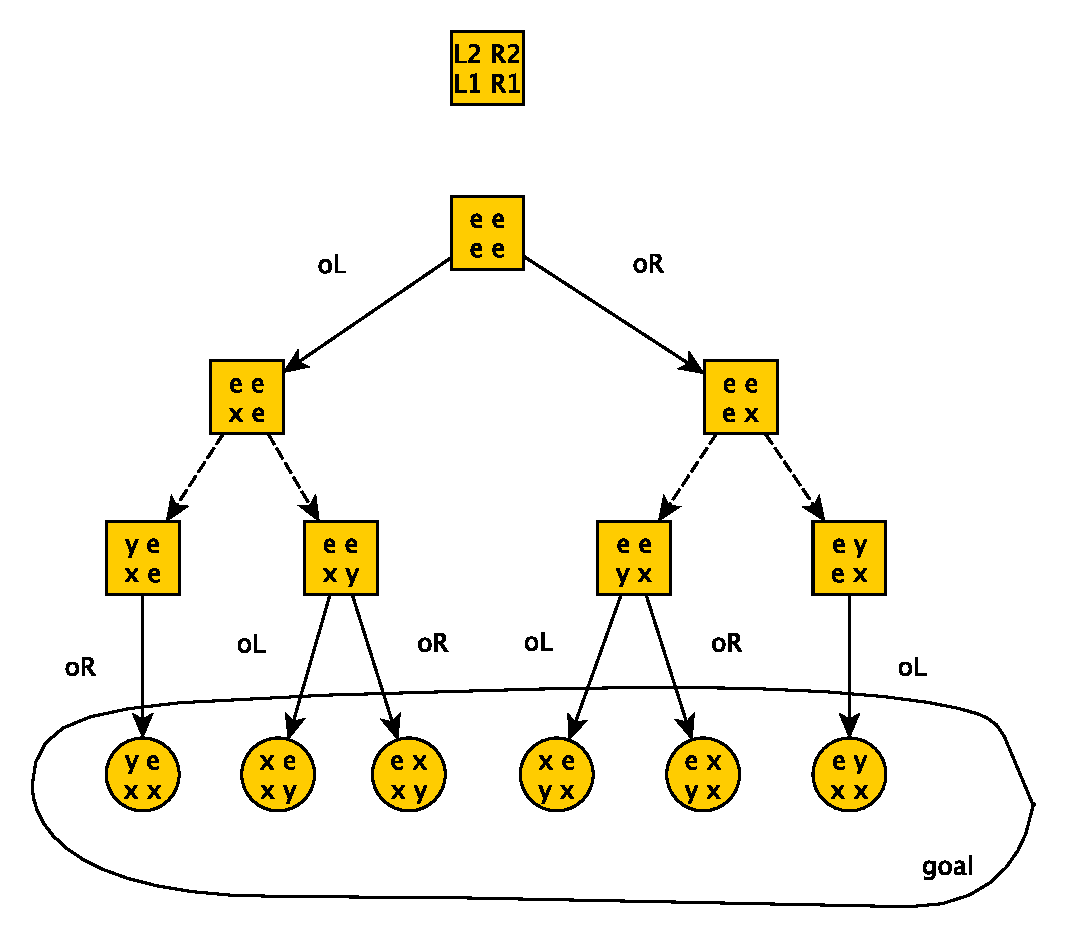
\includegraphics[scale=0.5]{NondeterministicTicTacToe}
\caption{Nondeterministic Transition Graph: TicTacToe}
\end{figure}



\label{lastpage}
\end{document}
